\documentclass[a4paper, 14pt]{extarticle}

% Поля
%--------------------------------------
\usepackage{geometry}
\geometry{a4paper,tmargin=2cm,bmargin=2cm,lmargin=3cm,rmargin=1cm}
%--------------------------------------


%Russian-specific packages
%--------------------------------------
\usepackage[T2A]{fontenc}
\usepackage[utf8]{inputenc} 
\usepackage[english, main=russian]{babel}
%--------------------------------------

\usepackage{textcomp}

% Красная строка
%--------------------------------------
\usepackage{indentfirst}               
%--------------------------------------             


%Graphics
%--------------------------------------
\usepackage{graphicx}
\graphicspath{ {./images/} }
\usepackage{wrapfig}
%--------------------------------------

% Полуторный интервал
%--------------------------------------
\linespread{1.3}                    
%--------------------------------------

%Выравнивание и переносы
%--------------------------------------
% Избавляемся от переполнений
\sloppy
% Запрещаем разрыв страницы после первой строки абзаца
\clubpenalty=10000
% Запрещаем разрыв страницы после последней строки абзаца
\widowpenalty=10000
%--------------------------------------

%Списки
\usepackage{enumitem}

%Подписи
\usepackage{caption} 

%Гиперссылки
\usepackage{hyperref}

\hypersetup {
	unicode=true
}

%Рисунки
%--------------------------------------
\DeclareCaptionLabelSeparator*{emdash}{~--- }
\captionsetup[figure]{labelsep=emdash,font=onehalfspacing,position=bottom}
%--------------------------------------

\usepackage{tempora}

%Листинги
%--------------------------------------
\usepackage{listings}
\lstset{
  basicstyle=\ttfamily\footnotesize, 
  %basicstyle=\footnotesize\AnkaCoder,        % the size of the fonts that are used for the code
  breakatwhitespace=false,         % sets if automatic breaks shoulbd only happen at whitespace
  breaklines=true,                 % sets automatic line breaking
  captionpos=t,                    % sets the caption-position to bottom
  inputencoding=utf8,
  frame=single,                    % adds a frame around the code
  keepspaces=true,                 % keeps spaces in text, useful for keeping indentation of code (possibly needs columns=flexible)
  keywordstyle=\bf,       % keyword style
  numbers=left,                    % where to put the line-numbers; possible values are (none, left, right)
  numbersep=5pt,                   % how far the line-numbers are from the code
  xleftmargin=25pt,
  xrightmargin=25pt,
  showspaces=false,                % show spaces everywhere adding particular underscores; it overrides 'showstringspaces'
  showstringspaces=false,          % underline spaces within strings only
  showtabs=false,                  % show tabs within strings adding particular underscores
  stepnumber=1,                    % the step between two line-numbers. If it's 1, each line will be numbered
  tabsize=2,                       % sets default tabsize to 8 spaces
  title=\lstname                   % show the filename of files included with \lstinputlisting; also try caption instead of title
}
%--------------------------------------

%%% Математические пакеты %%%
%--------------------------------------
\usepackage{amsthm,amsfonts,amsmath,amssymb,amscd}  % Математические дополнения от AMS
\usepackage{mathtools}                              % Добавляет окружение multlined
\usepackage[perpage]{footmisc}
%--------------------------------------

%--------------------------------------
%			НАЧАЛО ДОКУМЕНТА
%--------------------------------------

\begin{document}

%--------------------------------------
%			ТИТУЛЬНЫЙ ЛИСТ
%--------------------------------------
\begin{titlepage}
\thispagestyle{empty}
\newpage


%Шапка титульного листа
%--------------------------------------
\vspace*{-60pt}
\hspace{-65pt}
\begin{minipage}{0.3\textwidth}
\hspace*{-20pt}\centering

\includegraphics[width=\textwidth]{emblem}
\end{minipage}
\begin{minipage}{0.67\textwidth}\small \textbf{
\vspace*{-0.7ex}
\hspace*{-6pt}\centerline{Министерство науки и высшего образования Российской Федерации}
\vspace*{-0.7ex}
\centerline{Федеральное государственное бюджетное образовательное учреждение }
\vspace*{-0.7ex}
\centerline{высшего образования}
\vspace*{-0.7ex}
\centerline{<<Московский государственный технический университет}
\vspace*{-0.7ex}
\centerline{имени Н.Э. Баумана}
\vspace*{-0.7ex}
\centerline{(национальный исследовательский университет)>>}
\vspace*{-0.7ex}
\centerline{(МГТУ им. Н.Э. Баумана)}}
\end{minipage}
%--------------------------------------

%Полосы
%--------------------------------------
\vspace{-25pt}
\hspace{-35pt}\rule{\textwidth}{2.3pt}

\vspace*{-20.3pt}
\hspace{-35pt}\rule{\textwidth}{0.4pt}
%--------------------------------------

\vspace{1.5ex}
\hspace{-35pt} \noindent \small ФАКУЛЬТЕТ\hspace{80pt} <<Информатика и системы управления>>

\vspace*{-16pt}
\hspace{47pt}\rule{0.83\textwidth}{0.4pt}

\vspace{0.5ex}
\hspace{-35pt} \noindent \small КАФЕДРА\hspace{50pt} <<Теоретическая информатика и компьютерные технологии>>

\vspace*{-16pt}
\hspace{30pt}\rule{0.866\textwidth}{0.4pt}
  
\vspace{11em}

\begin{center}
\Large {\bf Лабораторная работа № 2} \\ 
\large {\bf по курсу <<Компьютерные сети>>} \\
\large <<Клиент и сервер HTTP>> 
\end{center}\normalsize

\vspace{8em}


\begin{flushright}
  {Студент группы ИУ9-32Б Волохов А. В. \hspace*{15pt}\\ 
  \vspace{2ex}
  Преподаватель Посевин Д. П.\hspace*{15pt}}
\end{flushright}

\bigskip

\vfill
 

\begin{center}
\textsl{Москва 2023}
\end{center}
\end{titlepage}
%--------------------------------------
%		КОНЕЦ ТИТУЛЬНОГО ЛИСТА
%--------------------------------------

\renewcommand{\ttdefault}{pcr}

\setlength{\tabcolsep}{3pt}
\newpage
\setcounter{page}{2}
\section{Задание}\label{Sect::task}
Целью данной работы является создание HTTP-клиента и HTTP-сервера на языке Go.
Формирование списка последних новостей с
https://www.baltimoresun.com/latest/
Исходный код программы представлен в листингах~\ref{lst:code1}--~\ref{lst:code2}--~\ref{lst:code3}.

\begin{figure}[!htb]
\begin{lstlisting}[language={Go},caption={download.go},label={lst:code1}]
package main

import (
	"github.com/mgutz/logxi/v1"
	"golang.org/x/net/html"
	"io"
	"net/http"
)

func getAttr(node *html.Node, key string) string {
	for _, attr := range node.Attr {
		if attr.Key == key {
			return attr.Val
		}
	}
	return ""
}

func isElem(node *html.Node, tag string) bool {
	return node != nil && node.Type == html.ElementNode && node.Data == tag
}

func isDiv(node *html.Node, class string) bool {
	return isElem(node, "div") && getAttr(node, "class") == class
}

type Item struct {
	Time, Title, SourceLink string
}

func search(node *html.Node) []*Item {
	var items []*Item

	if isElem(node, "article") && (getAttr(node, "class") == "container-fluid row flex_row " ||
		getAttr(node, "class") == "container-fluid row flex_row padding-sm-bottom") {
		item := &Item{}

		for a := node.FirstChild; a != nil; a = a.NextSibling {
			if isElem(a, "a") {
				item.SourceLink = "https://www.baltimoresun.com" + getAttr(a, "href")
				for c := a.FirstChild; c != nil; c = c.NextSibling {
					if isDiv(c, "headline-wrapper flex flex_col col-sm-xl-7") {
						for cChild := c.FirstChild; cChild != nil; cChild = cChild.NextSibling {
							if isElem(cChild, "div") &&
								(getAttr(cChild, "class") == "promo-headline font_20_custom font_mobile_custom "+
									"font_normal story-headline-link color_primary decoration_none  ") ||
								getAttr(cChild, "class") == "promo-headline font_18_custom font_mobile_custom "+
									"font_normal story-headline-link color_primary decoration_none  " {
								for tNode := cChild.FirstChild; tNode != nil; tNode = 

\end{lstlisting}
\end{figure}

\newpage

\begin{figure}[!htb]
\begin{lstlisting}[language={Go},caption={download.go - продолжение},label={lst:code2}]
tNode.NextSibling {
									if isElem(tNode, "h2") || isElem(tNode, "h1") {
										item.Title = tNode.FirstChild.Data
									}
								}
							} else if isElem(cChild, "div") && getAttr(cChild, "class") == "isDisabled" {
								for cChild2 := cChild.FirstChild; cChild2 != nil; cChild2 = cChild2.NextSibling {
									if isElem(cChild2, "div") && getAttr(cChild2, "class") == "padding-xs-top" {
										for tNode := cChild2.FirstChild; tNode != nil; tNode = tNode.NextSibling {
											if isElem(tNode, "time") {
												item.Time = getAttr(tNode, "datetime")
											}
										}
									}
								}}}}}}}
		items = append(items, item)
		log.Info("items:", "items", item)
	}

	for c := node.FirstChild; c != nil; c = c.NextSibling {
		childItems := search(c)
		if childItems != nil {
			items = append(items, childItems...)
		}
	}
	return items
}

func downloadNews() []*Item {
	log.Info("sending request to www.baltimoresun.com")
	if response, err := http.Get("https://www.baltimoresun.com/latest/"); err != nil {
		log.Error("request to baltimoresun.com failed", "error", err)
	} else {
		defer func(Body io.ReadCloser) {
			err := Body.Close()
			if err != nil {

			}
		}(response.Body)
		status := response.StatusCode
		log.Info("got response from www.baltimoresun.com", "status", status)
		if status == http.StatusOK {
			if doc, err := html.Parse(response.Body); err != nil {
				log.Error("invalid HTML from www.baltimoresun.com", "error", err)
			} else {
				log.Info("HTML from www.baltimoresun.com parsed successfully")
				return search(doc)
			}
		}
	}
	return nil
}
\end{lstlisting}
\end{figure}

\newpage
\begin{figure}[!htb]
\begin{lstlisting}[language={Go},caption={server.go},label={lst:code3}]
package main

import (
	"github.com/mgutz/logxi/v1"
	"html/template"
	"net/http"
)

const INDEX_HTML = `
    <!doctype html>
    <html lang="ru">
        <head>
            <meta charset="utf-8">
            <title>Последние новости с www.baltimoresun.com</title>
        </head>
        <body>
            {{if .}}
                {{range .}}
                    {{.Time}}
                    <a href="{{.SourceLink}}">{{.Title}}</a>
                    <br/>
                {{end}}
            {{else}}
                Не удалось загрузить новости!
            {{end}}
        </body>
    </html>
    `

var indexHtml = template.Must(template.New("index").Parse(INDEX_HTML))

func serveClient(response http.ResponseWriter, request *http.Request) {
	path := request.URL.Path
	log.Info("got request", "Method", request.Method, "Path", path)
	if path != "/" && path != "/index.html" {
		log.Error("invalid path", "Path", path)
		response.WriteHeader(http.StatusNotFound)
	} else if err := indexHtml.Execute(response, downloadNews()); err != nil {
		log.Error("HTML creation failed", "error", err)
	} else {
		log.Info("response sent to client successfully")
	}
}

func main() {
	http.HandleFunc("/", serveClient)
	log.Info("starting listener")
	log.Error("listener failed", "error", http.ListenAndServe("127.0.0.1:6060", nil))
}

\end{lstlisting}
\end{figure}

\newpage

\begin{figure}[!htb]
	\centering
	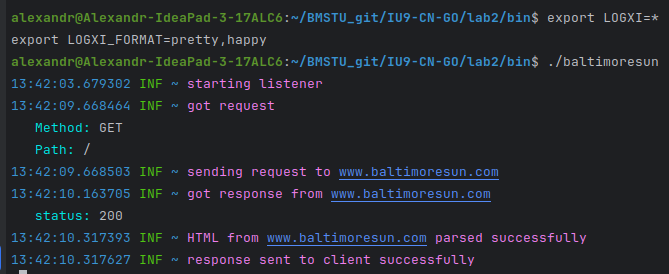
\includegraphics[width=0.8\textwidth]{res.png}
\caption{Пример работы сервера}
\label{fig:img1}
\end{figure}

\end{document}
